\section{Design of \sys}
\label{s:impl}

\sys is a coverage-directed concurrency fuzzer to effectively discover
concurrency bugs.
%
The key improvement of \sys lies in adopting interleaving segment
coverage and the coverage-directed interleaving \dr{}mutation
algorithgm described in \autoref{s:design}.
%




In the following of subsections, we describe design details of the
userspace fuzzer~(\autoref{ss:fuzzer}), the target kernel
instrumentation~(\autoref{ss:instrumentation}), the execution
engine~(\autoref{ss:engine}), and the implementation details of
\sys~(\autoref{ss:impl}).


\subsection{Target Kernel Instrumentation}
\label{ss:instrumentation}

\sys requires to profile basic blocks and memory accesses executed by
each system calls.
%
To this end, \sys incorporates a compiler pass that inserts callback
function calls 1) at the beginning of each basic block, and 2) before
each instruction that accesses globally-visible memory objects.
%
These callback functions trace basic blocks and memory accesses during
the execution in the kernel, and records them into memory regions
shared between the user space and the kernel space.



\begin{figure}
  \centering
  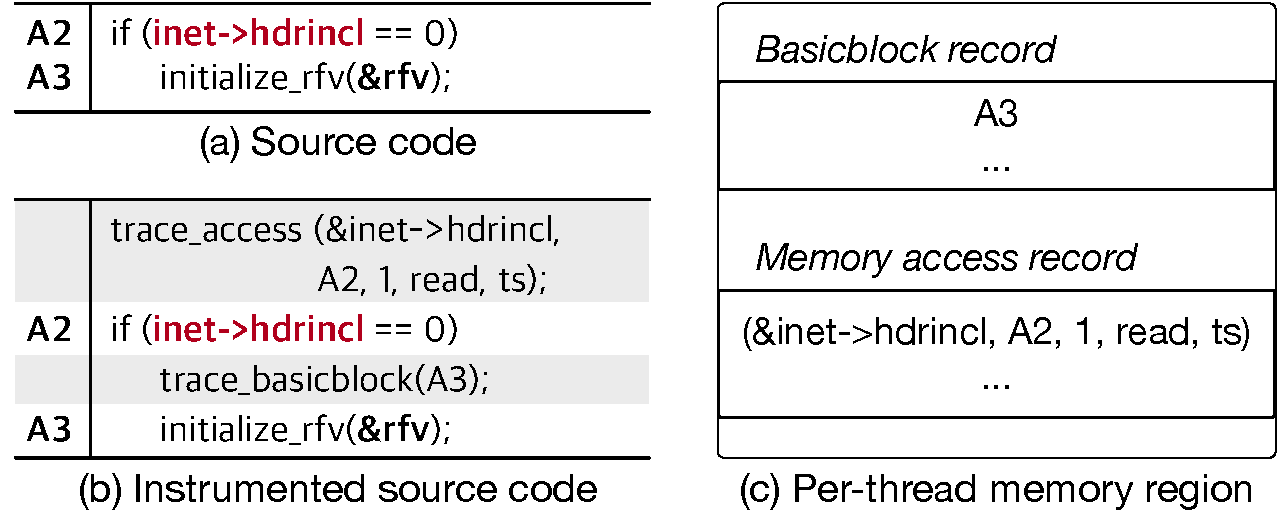
\includegraphics[width=\linewidth]{fig/instrumentation.pdf}
  \caption{}
  \label{fig:instrumentation}
\end{figure}

\autoref{fig:instrumentation} shows how the \sys's compiler pass
works.
%
When compiling a source code, the compiler pass inserts a function
call \texttt{trace_basicblock()} at the beginning of the basic block
(\ie, \texttt{0xb}) .
%
Similarly, a function call \texttt{trace_read()} is also inserted at
\texttt{0x0} before an instruction at \texttt{0x5} that access
globally-visible memory objects (\eg, at \texttt{0x0}).


During runtime, the callback function \texttt{trace_basicblock()}
records starting address of each basic block (\eg, \texttt{0xb}) into
a memory region \texttt{Basicblock record}.
%
Also, callback functions \texttt{trace_read()} and
\texttt{trace_write()} record a four-tuple of the instruction address,
the memory object addresss, the size of memory access, and the type of
memory access (\eg, \texttt{(\&inet->hdrincl, 0x5, 1, read)}, into
\texttt{Memory access record}.


It is worth noting that \texttt{Basicblock record} and \texttt{Memory
  access record} are per-thread memory regions which is shared with
the userspace space and the kernel space, so threads of the userspace
fuzzer can identify basic blocks and memory accesses they executed.









% Unlike data race detectors such as KCSAN~\cite{kcsan}, the \sys's
% scheduling mechanism needs to recognize both plane memory accesses and
% annotated memory accesses such as atomic operations.
% %
% We deal with these two types of accesses differently since annotated
% accesses usually are implemented in assembly code, which is hard for a
% LLVM pass to understand.
% %
% In order to instrument plane accesses, we implement a LLVM pass that
% insert callback function calls after memory accesses on LLVM IR.
% %
% Our pass runs after most of binary transfomration is done, so it
% \XXX{...}.
% %
% For annotated instructions, we rely on the functionality of
% KASAN~\cite{kasan} to instrument atomic operations.
% %
% KASAN provides wrapper functions of annotation APIs to call callback
% functions before annotated memory operations, and we instruct the
% wrapper functions to call our callbacks as well.
% %
% Our callbcak functions write memory access operations along with
% various information into a region mmap-ed shared region shared by a
% userspace program (\ie, fuzzer) and a kernel. The information about
% memory operations includes the instruction address, the start address
% of a memory location, and the size of memory access.
% %
% Accordingly, a fuzzer is able to identify what memory access
% operations took place during the execution.

% \sys also requires an additional module called a trampoline that is
% used to suspend and resume a running thread. Details about the
% trampoline are described in \autoref{ss:engine}.


\subsection{Execution Engine}
\label{ss:engine}

\begin{figure}
  \centering
  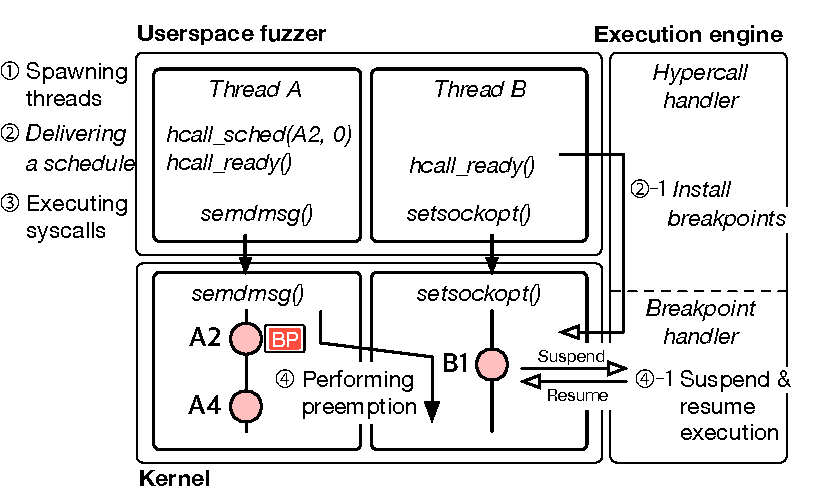
\includegraphics[width=0.9\linewidth]{fig/workflow-hypervisor.pdf}
  \caption{The workflow of the execution engine. \red{IMPORTANT: this
      is copied from AITIA. Need to redraw}}
  \label{fig:workflow-hypervisor}
\end{figure}

We introduce an execution engine in order to allow the userspace
fuzzer to control thread scheduling.
%
The execution engine is implemented in the hypervisor layer to be
non-intrusive to the execution of the kernel, and communicates with
the userspace fuzzer through hypercall interfaces.



\PP{Schedule}
%
A schedule describes





\PP{Enforcing interleavings}
%
\autoref{fig:workflow-hypervisor} shows a workflow of the execution
engine.
%
The userspace fuzzer spawns threads that execute a system call
respectively.
%
Then, each thread calls hypercalls to deliever scheduling points to
the execution engine before executing a system call.



After the fuzzer sends a schedule, the userspace fuzzer notifies the
execution engine, and the execution engine starts executing with the
intial thread specified in the given schedule while other threads are
suspended.

%
When the running thread reaches a scheduling point, a hypervisor
performs preemption by suspending the running thread and resuming the
next thread to run in order to enforce the execution order between
memory access operations.
%
\dr{TODO:}
Details about suspending and resuming a thread is described later.


\PP{Suspending a thread}
%
A few prior approaches~\cite{ski, snowboard, razzer} suspend a vCPU
instead of a guest thread. While suspending a vCPU grants the ability
to control an interleaving, it is not suitable for our purpose because
suspending a vCPU may unexpectedly suspend another vCPU. An example we
observed is TLB shootdown~\cite{tlbshootdown}. When a vCPU wants TLB
shootdown, it sends inter-process interrupts (IPIs) to all cores and
wait until all cores to execute the TLB shootdown handler.  In this
case, if one vCPU is entirely suspended, the TLB shootdown cannot be
successfully conducted causing the vCPU invoking TLB shootdown
blocked.
%
Therefore, instead of adopting the prior approach, our hypervisor is
designed to suspends and resumes a guest thread.
%
In order to suspend a thread at an arbirary location, we use a
hardware breakpoint functionality~\cite{hwbp} shipped in modern Intel
CPU chipsets.
%
When a guest thread hits a breakpoint, our hypervisor saves its
register values and then changes the program counter of the thread to
an infinite loop called trampoline. In the trampoline, the thread
keeps calling \texttt{cond_resched()} to yield a CPU to make all other
kernel functionalities (\eg, handling the TLB shootdown handler) work
normally. When the guest thread resumes, our hypervisor restores
registers with the values saved when the thread is suspended, and the
thread continues its execution.


\PP{Virtual Machine Instrospection}
%
\dr{Not important contents but too long}
%
In the middle of execution, our hypervisor introspects the target
kernel for two reasons.
%
First, when a breakpoint is hit, it needs to determine whether the
breakpoint is hit by a fuzzer-controlled thread.
%
As a hardware breakpoint does not distinguish the running context of a
kernel, if the context switch happens, a breakpoint may be hit by
another thread or an interrupt handler, making the execution out of
expectation.
%
The hypervisor recognizes a running context using \texttt{task_struct}
which holds the thread description, and the per-cpu
\texttt{preempt_count} variable indicating what context the thread is
in (\eg, a task context for running a syscall, or a hardIRQ context to
handle hardware interrupts).
%
If a breakpoint is hit by a context other than the fuzzer-controlled
thread, our hypervisor ignores it and keeps the breakpoint.

Second, when a running thread tries to acquire a lock, our hypervisor
inspects the lock is held by a suspended thread.
%
When the suspended thread already acquires a lock while the running
thread wants to hold the same lock, the whole execution cannot make a
progress, because our hypervisor forces the lock-holding thread to
suspend.
%
Therefore, our hypervisor inspects whether the running thread is going
to be blocked due to the lock contention, and if it is, our hypervisor
takes control from the running thread to the suspended thread.
%
Inspecting the lock contention is conducted by hooking lockdep
functions~\cite{lockdep} that are commonly called from synchronization
prmitives.
%
When the lockdep functions are called, our hypervisor determins
whether the running thread can make a progress through various
information such as the address of the synchronization primitive, and
operation type (\ie, lock, unlock, and trylock).

\subsection{Userspace Fuzzer}
\label{ss:fuzzer}



\begin{figure}
  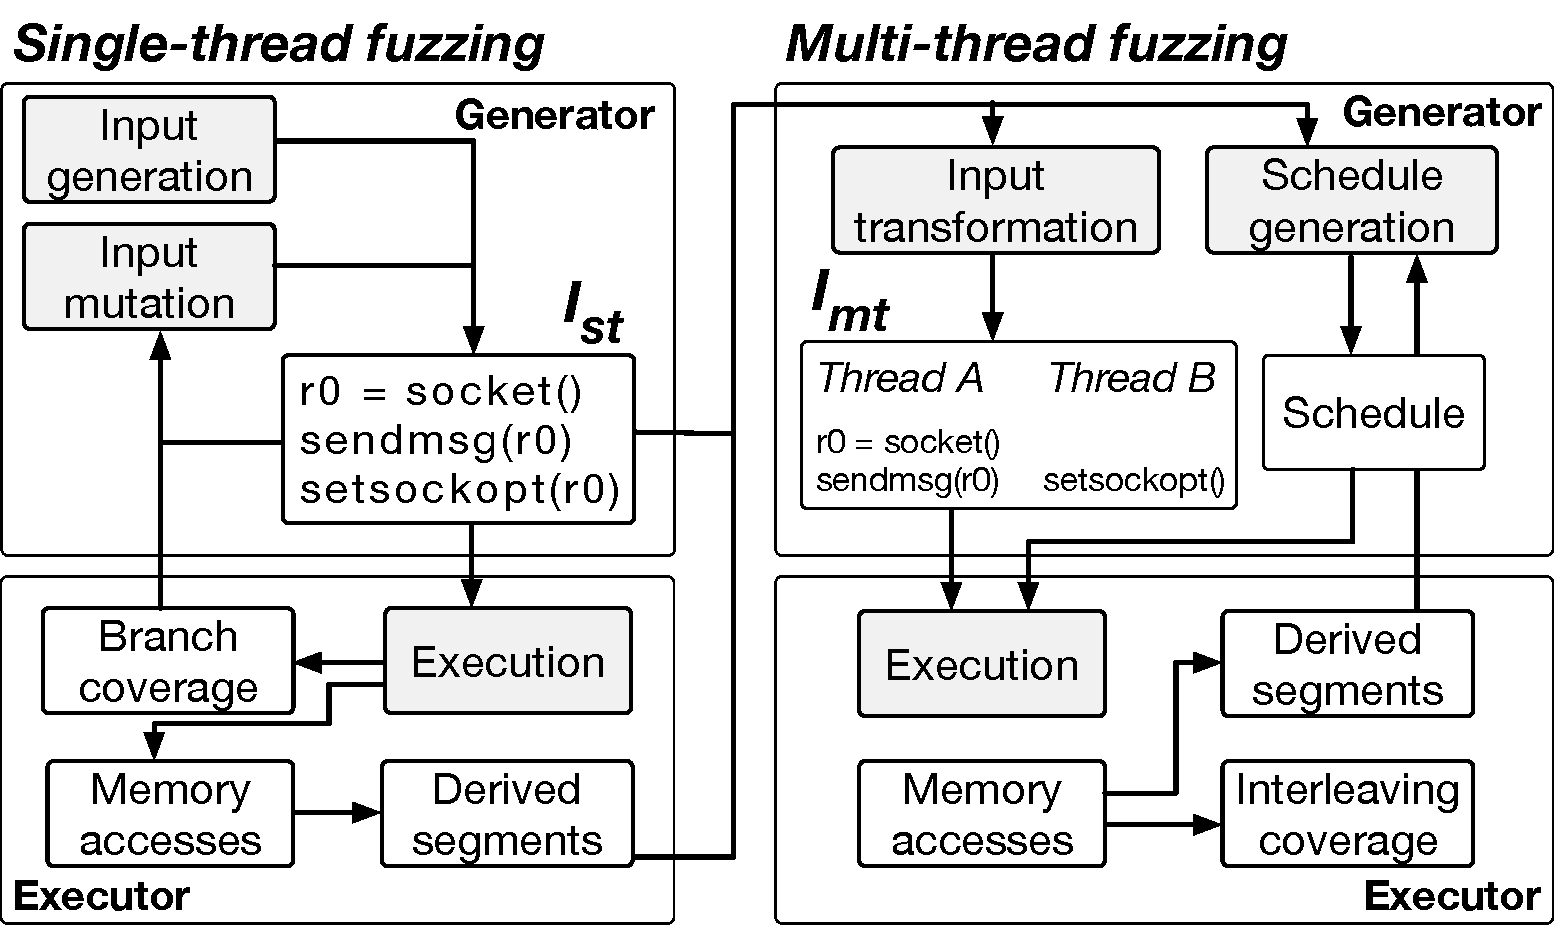
\includegraphics[width=0.9\linewidth]{fig/architecture.pdf}
  \caption{Workflow of \sys \dr{TODO: redraw to describe the workflow}}
  \label{fig:workflow}
\end{figure}


The \sys's userspace fuzzer conducts two-stage pipelined fuzzing
similar with recent concurrency fuzzers, Razzer~\cite{razzer} and
Snowboard~\cite{snowboard}.
%
In \sys, the first stage is a \textit{single-thread} fuzzing that
focuses on expanding code coverage, and the second stage is a
\textit{multi-thread} fuzzing to explore thread interleavings.

Both stages consists of two components, an input generator and an
input executor. We explain details of each component in the following.


\subsubsection{Single-thread fuzzing}
%
In a single-thread fuzzing phase, the single-thread generator
generates a single-thread input (refered as $I_{ST}$) in the form of a
sequence of random system calls.
%
And then, the single-thread executor executes $I_{ST}$ to perform two
things.
%
First, it collects code coverage of $I_{ST}$ with the purpose of
exploring source codes residing deep inside the kernel.
%
Second, it identifies two system calls in $I_{ST}$ that potentially
exhibit new interleaving coverage.  If identified, $I_{ST}$ will be
handed to the next phase, namely the multi-thread fuzzing.


\PP{Single-Thread Generator}
%
The single-thread generator is similar with conventional
fuzzing~\cite{syzkaller}.
%
It constructs a single-threaded system call sequence $I_{ST}$ with two
strategies: generation and mutation.
%
When using the generation strategy, \sys randomly generates a system
call sequence based on well-formed system call description grammar
\texttt{Syzlang}~\cite{syzlang}.
%
\texttt{Syzlang} describes templates of available system calls
including types of arguments and the type of a return value, as well
as a range of feasible values of each arguments.
%
According to \texttt{Syzlang}, \sys produces a single-thread system
call sequence by repeatedly selecting a random system call and
providing reasonable arguments of the system call.

The mutation strategy is an alternative of the generating strategy.
When using a mutation strategy, \sys picks up a already-generated
single-thread input, and modifies the single-thread input by appending
additional system calls, removing existing system calls, or changing
values of arguments of existing system calls.


\PP{Single-Thread Executor}
%
Given $I_{ST}$ from the single-thread generator, the single-thread
executor runs $I_{ST}$, and profiles basic blocks and memory accesses
executed by each system call with a support from instrumentation
detailed in \autoref{ss:instrumentation}.

With profiled basic blocks and memory accesses, the single-thread
executor conducts two tasks.
%
The first task is similar with what conventional kernel fuzzing
does.
%
In other words, the single-thread executor computes branch coverage
using profiled basic blocks.
%
Then, if $I_{ST}$ exposes new branch coverage that has not been
explored, \sys keeps $I_{ST}$, and feeds it back to the single-thread
generator so that the single-thread generator further mutates $I_{ST}$
to find more branch coverage.
%
As a result, \sys keeps a minimal set of $I_{ST}$, called a corpus,
which may execute previously-executed branches when running
single-thread inputs in the corpus.


Second, the single-thread executor identifies a pair of system calls
in $I_{ST}$ potentially exposes new interleaving coverage if executed
concurrently.
%
More specifically, for each pair of system calls, the single-thread
executor checks  \dr{}
%



\subsubsection{Multi-thread fuzzing}
%
After $I_{ST}$ is handed with a pair of system calls to execute
concurrently, the multi-thread generator transforms $I_{ST}$ to a
multi-thread input $I_{MT}$.
%
In addition, the multi-thread generator generates \textit{schedules}
where each schedule describes how to enforce thread interleaving (\ie,
a set of scheduling points) during runtime.


The multi-thread executor then repeatedly tests each schedule of
$I_{MT}$ one at a time.
%
To this end, the multi-thread executor instruments $I_{MT}$ with
hypercalls in order to tell the execution engine how to control thread
scheduling.
%
Lastly, the multi-thread executor runs $I_{MT}$ while enforcing a
given schedule with a support of the execution
engine~(\autoref{ss:engine}).




\PP{Multi-Thread Generator}
%
% In order to use interleaving graph as interleaving coverage, we need a
% method to store them, and compare them to a new interleaving graph.
% %
% We choose to use a hash value of

% the FNV-1~\cite{fnv, fnv-go}, non-cryptographic hash function,


% A schedule is an outcome of the interleaving mutation.
% A schedule contains an initial thread, and a set of scheduling points
% indicating an instruction on which preemption occurs.


With a given $I_{ST}$ and a pair of system calls, the multi-thread
generator transforms it to $I_{MT}$.




\PP{Multi-Thread Executor}
%
A 





\subsection{Implementation}
\label{ss:impl}

We implement \sys in various software layers.
%

%
To allow 


We use scc~\cite{scc} and sloccount~\cite{sloccount} to measure LoC of
GO and C respectively.


%%% Local Variables:
%%% mode: latex
%%% TeX-master: "p"
%%% End:
